\documentclass[a4paper,10pt]{report}
\usepackage[a4paper,width=150mm,top=25mm,bottom=25mm]{geometry}
\usepackage[export]{adjustbox}
\usepackage[utf8]{inputenc}
\usepackage{xspace}
\usepackage[portuguese]{babel}

% o comando say
\usepackage{dirtytalk}

%para que o primeiro paragrafo indente
\usepackage{indentfirst}

%Fontes especias de matemática
\usepackage{amsfonts}

%hide hilelinks esconde os links de terem bordas feias
\usepackage[hidelinks]{hyperref}
% pacote para os headers e footers fixes
\usepackage{fancyhdr}


%para poder ter os compactitem lists
\usepackage{paralist}

%ter acesso a imagens
\usepackage{graphicx}
\graphicspath{{images}}

\usepackage{setspace}
\usepackage{afterpage}
% CORES

%tratar das cores
\usepackage{xcolor}
\usepackage{pagecolor,lipsum}% http://ctan.org/pkg/{pagecolor,lipsum}

% definição de uma cor
% \definecolor{name}{model}{color-spec}
\definecolor{aquamarine}{rgb}{0, 181, 190}


\usepackage{xcolor}
\usepackage{todonotes}
\usepackage{biblatex}
\addbibresource{referencias.bib}

%MACROS
\newcommand{\lk}[2]{\href{#1}{\textcolor{aquamarine}{#2}}}
\newcommand{\chapterf}[1]{\chapter{#1}\thispagestyle{fancy}}


% Informações do autor
\newcommand{\myauthor}{[NOME COMPLETO DO ALUNO]}
\newcommand{\mynumerodealuno}{[NUMERO DE ALUNO]}

%valores da palestra
\newcommand{\palestratitulo} {[TITULO DA PALESTRA]}
\newcommand{\palestraautor} {[NOMES DOS AUTORES]}
\newcommand{\palestradata} {[DATA DA PALESTRA]}
\newcommand{\palestranumero} {[NUMERO DA PALESTRA]}

% set dos headers e footers
\pagestyle{fancy}
\fancyhf{}
\renewcommand{\headrulewidth}{0pt}
\rfoot{\thepage}



%set do espaçamento entre linhas
\setstretch{1.25}
%set indentação
\setlength\parindent{0.75cm}

%set font family to arial
\usepackage{helvet}
\renewcommand{\familydefault}{\sfdefault}

\newcommand \mytitle {Relatório da Palestra nº \palestranumero}

\title{\mytitle}
\author{\myauthor}

\newcommand\myemptypage{
    \newpage
    \null
    \thispagestyle{empty}
    \addtocounter{page}{-1}
    \newpage
    }


\begin{document}
\begin{titlepage}
    $\vcenter{\hbox{{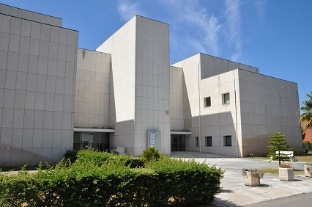
\includegraphics[width=0.4\textwidth]{DEIS}}}}%
    \vcenter{\begin{minipage}{0.5\textwidth}\centering    
            \begin{flushright}
            \textbf{Departamento de Engenharia Informática e de Sistemas}\\
            \textbf{Instituto Superior de Engenharia de Coimbra}
            Instituto Politécnico de Coimbra
        \end{flushright}
    \end{minipage} }$
    \begin{center}
        \vspace{0.5cm}
        \begin{large}
            \newcommand{\spacetitle}{0.0cm}

            Licenciatura em Engenharia Informática
            \vspace{\spacetitle}

            Ramo de Redes e Administração de Sistemas
            \vspace{\spacetitle}

            Unidade Curricular de Ética e Deontologia
            \vspace{\spacetitle}

            Ano Letivo de 2021/2022
            \vspace{\spacetitle}

            \vfill

            Palestra nº \palestranumero
            \vspace{\spacetitle}

            \palestratitulo
            \vspace{\spacetitle}

            Realizado por \palestraautor

            Realizada em \palestradata

            \vfill

            
\includegraphics[width=0.4\textwidth]{ISEC}
            \vfill

            \myauthor

            Número de Aluno: \mynumerodealuno

            Coimbra, \today
            \vspace{\spacetitle}

            \myauthor

        \end{large}
    \end{center}
\end{titlepage}

\thispagestyle{empty}

\begin{center}
    \textbf{[AUTOR DO RELATORIO]}\\
    \vspace*{\stretch{1}}
    \textbf{[TITULO]}\\
    \vspace*{\stretch{1}}
    \vspace*{\fill}
    \textbf{Coimbra, \today}
\end{center}


\tableofcontents{}
\thispagestyle{empty}

\newpage{}

\pagenumbering{roman}
\section*{Resumo}
\addcontentsline{toc}{chapter}{Resumo}
\paragraph{}
Apresente uma síntese do conteudo do relatorio, destacando os aspetos mais relevantes, a partir dos quais retire as palavras chave


\myemptypage{}

\pagenumbering{arabic}
\chapterf{Introdução}
\paragraph{}
Inserir número da página no canto inferior direito. Iniciar com o número 1 em arábico.
Faça uma apresentação do assunto, oferecendo ao leitor uma ideia do todo a ser relatado, sem entrar em maiores detalhes.\\

A sua redacção deve contemplar os seguintes aspectos\\
- o tema abordado na palestra;\\
- qual a sequência seguida no seu Relatório;\\
- o que espera com o referido Relatório;\\
- as partes que compõem o Relatório.\\

Formatação do texto:\\
- Fonte: 12 pt, Arial, Justificado.\\
- Entre linhas: Single\\
- Entre parágrafos: 12 pt after; before 0 pt\\
- Avanço da Primeira Linha: 0,75 cm\\


Os novos capítulos têm de começar numa folha ímpar!\\
Exceptuando as folhas referentes às capas, folha de rosto, de índices e do resumo, o texto referente ao relatório deverá ter no mínimo 8 páginas!\\
Use o texto constante destas notas como modelo para a formatação do texto do seu relatório!\\

\chapterf{Descrição do Tema Abordado na Palestra}

\section{Nome do Tema}

Descreva com clareza, objectividade e detalhes os principais aspectos que foram focados na palestra e o porquê da escolha desses aspectos sobre o tema exposto. 
Pesquise e apresente fundamentos teóricos referidos pelo palestrante neste seu relatório.
Refira os principais linhas de pensamento seguidas na palestra pelo apresentador!


\section{Secção 2.2}
[CONTEUDO]
\newpage

%critica
\chapterf{Análise Crítica}

\section{Secção 3.1}

Tomando por base o que o palestrante apresentou e eventuais fontes que tenha encontrado em pesquisa sobre o tema, exponha livremente, com clareza e objectividade, a sua posição sobre o assunto abordado, fazendo uma análise critica de acordo com a sua opinião sobre o assunto e do que foi exposto na palestra. 
Fundamente a sua posição sobre o assunto apresentado na palestra! 

\chapterf{Considerações Finais}
Tomando por base as etapas anteriores, escreva livremente, com clareza e objectividade, as conclusões que tirou do que foi exposto na palestra, a análise do tema por parte do palestrante, procure avaliar de modo crítico, reflexivo e argumentativo o tema apresentado e a um resumo da sua visão critica do que foi exposto e do tema em si.

\newpage{}

\section*{Referências}
\pagestyle{fancy}
\addcontentsline{toc}{chapter}{Referências}
Para a inserção de referências, siga a notação APA.  O Word permite a inserção automática de referências com  esta notação

\newpage{}
\pagenumbering{Alph}
\section*{Anexos}
\addcontentsline{toc}{chapter}{Anexos}

\end{document}